\chapter{Proceso de negocio. Fundamentos teóricos}
\label{chap:teoria}

\lettrine{A} {día} de hoy es innegable el papel crucial que juegan las tecnologías de la información en general y los sistemas de información en particular dentro de la gestión de procesos de negocio de cara a la consecución de objetivos de forma eficaz y eficiente. 

El mercado está en continua evolución. Los sistemas de información nos proporcionan la tecnología básica necesaria tanto para crear nuevas funcionalidades como para adaptar las existentes para poder satisfacer las nuevas necesidades que van surgiendo. 


Este capítulo pretende ser una aproximación tanto a los conceptos teóricos en los que se enmarcan los procesos empresariales dentro del sector \acrfull{tic} (entre los que se engloba el mantenimiento del catálogo de servicios y la contratación de los mismos) como a los conceptos manejados por la herramienta desarrollada en este \acrshort{tfg}, que, como ya hemos dicho, es una aplicación para la gestión y el mantenimiento del catálogo de servicios y las contrataciones de una empresa.


\section{Proceso de negocio}

Hammer \& Champy (1993)~\cite{Hammer-Champy} definieron el proceso de negocio como:

\begin{displayquote}
\textquote{Una colección de actividades que toman uno o más tipos de entradas y crean una salida que tiene valor para el cliente}. 
\end{displayquote}

Así pues, podemos entender un proceso de negocio como un conjunto de funciones dentro de una secuencia específica que proporciona valor a un cliente interno o externo y cada función dentro de un proceso puede ser a su vez interpretada como un proceso en si mismo llamado sub-proceso. El desencadenante de este sub-proceso es el proceso previo (o el evento inicial que da comienzo al proceso en general) y devuelve un resultado de valor para el siguiente proceso o para el cliente final y sus procesos si este es el último sub-proceso de un proceso de extremo a extremo~\cite{Kirchmer}. 

Esta descomposición de procesos en sub-procesos puede extenderse tanto
como las funciones resultados sigan teniendo sentido desde el punto de
vista de negocio: por ejemplo el sub-proceso ``gestión de ventas'' puede describirse en detalle usando funciones como ``registro de orden de venta'' o ``asignación de productos a la orden de venta'', sin embargo descomponer la función ``registro de orden de venta'' en actividades como ``introducir nombre de cliente'', ``introducir dirección de cliente'', etc. no aportan relevancia alguna desde el punto de vista de negocio.

Con el objetivo de poder definir de forma sencilla los procesos más complejos sin dejar de lado ningún aspecto importante de los mismos surge la \acrfull{aris}, una aproximación al proceso de arquitectura y modelado empresarial desarrollado por August-Wilhem Scheers y que permite describir un proceso de negocio desde cinco puntos de vista diferentes, dando respuesta a todas las cuestiones relevantes relativas al proceso:
\begin{itemize}
\item Vista organizacional: ¿quién (gente, departamentos, empresas, etc.) está involucrado en el proceso?
\item Vista funcional: ¿qué funciones se llevan a cabo dentro del proceso?
\item Vista de datos: ¿qué datos o información es necesaria/producida para/en el proceso?
\item Vista de entrega: ¿qué son los entregables del proceso y por qué los necesito?
\item Vista de control: el cómo se ve en conjunto refleja el quién está haciendo qué, qué datos producen entregables y cuál es la secuencia lógica que hace que las funciones lleven a cabo su función.
\end{itemize}


La \figurename~\ref{fig:aris} muestra la arquitectura \acrshort{aris}.
El elemento más importante de la arquitectura es la vista de control. Esta muestra cómo dos o más aspectos de un proceso se relacionan, por ejemplo quién es responsable de una función determinada o qué función usa determinados datos. La vista resultado de la integración de varios aspectos del proceso de negocio es la llave para la gestión exitosa de dichos procesos. \acrshort{aris} ayuda a convertir los procesos en algo \textit{tangible} al definir cómo describirlos asentando la base para convertir la \acrfull{bpm} en una disciplina de gestión real.

\begin{figure}
  \centering
  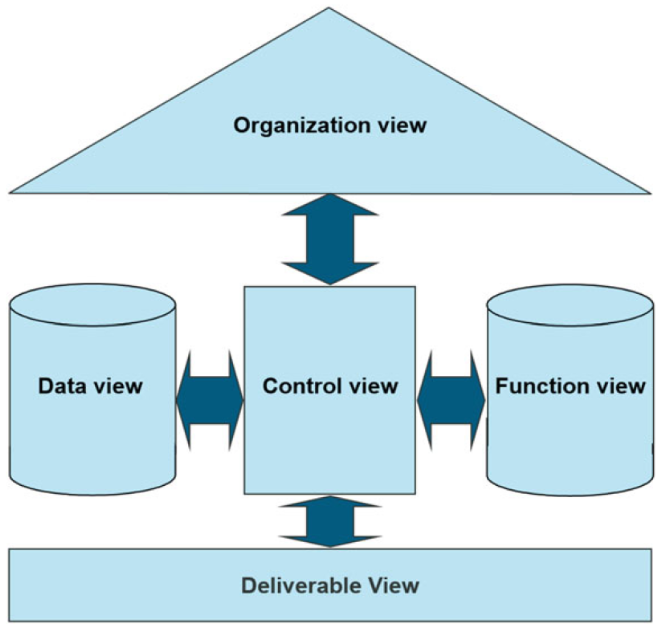
\includegraphics[width=0.45\textwidth]{imaxes/aris.png}
  \caption{Arquitectura de sistema de información integrada (\acrshort{aris}): sus vistas y las relaciones entre ellas.}
  \label{fig:aris}
\end{figure}


\subsection{Gestión de proceso de negocio (BPM)}

Una \acrshort{bpm} incluye conceptos, métodos y técnicas para soportar el diseño, la administración, la configuración, la representación y el análisis de los procesos de negocio~\cite{Weske}.
La base del \acrshort{bpm} es la representación explícita de los procesos de negocio con sus actividades y las restricciones de ejecución de los mismos.
El ciclo de vida de \acrshort{bpm} consta de cinco fases~\cite{bpmLifecycle}, tal y como se muestra en la \figurename~\ref{fig:lifecycle-bpm}.

\begin{figure}
  \centering
  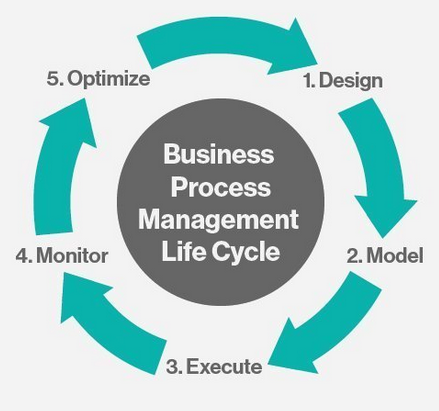
\includegraphics[width=0.30\textwidth]{imaxes/bpm-lifecycle.png}
  \caption{Ciclo de vida del \acrshort{bpm}}
  \label{fig:lifecycle-bpm}
\end{figure}

\begin{enumerate}
\item \textbf{Diseño}: abarca tanto la identificación de procesos existentes como el diseño de procesos ``futuros''. El objetivo es garantizar un diseño correcto y eficiente. Debe haber una sincronización entre los procesos existentes y el diseño de un nuevo proceso para evitar posibles interrupciones.
\item \textbf{Modelado}: se crea una representación visual del modelo de proceso. Esto debe incluir detalles específicos, como líneas de tiempo, descripciones de tareas y cualquier flujo de datos en el proceso. 
\item \textbf{Ejecución}: consiste en una prueba de concepto, probando el nuevo sistema BPM con un grupo limitado. Después de incorporar cualquier comentario, el equipo puede comenzar a implementar el proceso a un público más amplio.
\item \textbf{Supervisión}:  durante esta etapa, se supervisa el proceso, se miden las mejoras en la eficiencia y se identifica cualquier cuello de botella adicional.
\item \textbf{Optimización}: se realizan los ajustes finales al proceso para mejorar la actividad empresarial.
\end{enumerate}

Entre las ventajas que proporcionan los \acrshort{bpm} se encuentran las siguientes:
\begin{itemize}
\item Mayor eficiencia y ahorro de costes: gracias a la optimización de los procesos existentes y a la incorporación de más estructura en el desarrollo de nuevos procesos, eliminando redundancias y cuellos de botella.
\item Mejor experiencia de empleados y clientes: ya que permite eliminar el trabajo repetitivo y aumentar la accesibilidad de la información mejorando la productividad y la implicación con el cliente.
\item Procesos más escalables: a través de la mejora en la ejecución de procesos y la automatización de flujos de trabajo se facilita el escalado de procesos a otras zonas geográficas de todo el mundo.
\item Mayor transparencia: puesto que la automatización de procesos de negocio define claramente a los propietarios para las tareas a lo largo del proceso, se proporciona más transparencia y responsabilidad a lo largo de un proceso determinad, favoreciendo la comunicación entre equipos.
\end{itemize}




\section{Sistemas de soporte operacional y Sistemas de soporte de negocio}

Centrándonos en el área de las telecomunicaciones, nos encontramos con dos nuevos conceptos:


\acrfull{oss}. Se trata de un término usado para describir los sistemas de procesado de información utilizados por las operadoras para gestionar sus redes de comunicación. Ayudan a las operadoras a diseñar, construir, operar y mantener las redes de comunicaciones.

\acrfull{bss} es el término tradicionalmente utilizado para describir las funcionalidades de negocio y/o orientadas al cliente. Estas herramientas  permiten que una organización contacte con sus clientes, crear ofertas para ellos, emitir facturas así como transacciones entre operadores de comunicaciones (liquidaciones, punto de interconexión, etc.). Es aquí donde se enmarcan las soluciones software \acrshort{crm} y \acrshort{erp}.

De forma conjunta \acrshort{oss} y \acrshort{bss} permiten a los operadores de red ofrecer servicios de manera eficiente y confiable a un enorme número de suscriptores en algunas de las máquinas más complejas del mundo, las redes globales de telecomunicaciones.




\section{Gestión de relaciones con los clientes y Sistema de Planificación de recursos empresariales}

En esta sección describiremos las dos plataformas de software que son el referente de las soluciones empresariales.

A día de hoy ambas plataformas guardan muchas similitudes, aunque cada una tiene su propio punto de vista acerca de la solución aportada:
\begin{itemize}
\item El \acrshort{crm} se centra mejorar las ventas .
\item El \acrshort{erp} tiene como objetivo reducir costes aumentando la productividad.
\end{itemize}



\subsection{CRM}
\label{sub:crm}

Un \acrfull{crm} es una estrategia comercial que optimiza los ingresos y la rentabilidad al tiempo que promueve la satisfacción y la lealtad del cliente. Las tecnologías CRM permiten la estrategia de relación con los clientes al tiempo que identifican y gestionan esas relaciones~\cite{GartnerCRM}. 

Así pues el conjunto de conceptos, procedimientos y reglas que una empresa sigue para comunicarse con sus consumidores se conocen como  \acrshort{crm} y por definición cubre todas las formas en las que se administran las relaciones con los clientes en los distintos ámbitos empresariales: ventas, marketing, servicio al cliente y comercio electrónico~\cite{SAP-CRM} . 

Por lo general, cuando hablamos de \acrshort{crm} estamos refiriéndonos a los sistemas de software que nos ayudan a construir estrategias de negocio para retener y captar clientes.
El software \acrfull{crm} permite automatizar e integrar estas actividades orientadas al cliente e incluso pueden ofrecer herramientas para el análisis de clientes, la personalización, las redes sociales, la colaboración y mucho más. La funcionalidad que el software \acrshort{crm} proporciona a las empresas se divide en cuatro segmentos: ventas, marketing, servicio al clientes y comercio digital~\cite{GartnerCRM}. 


\subsection{ERP}
\label{sec:erp}
Un \acrfull{erp} se define como la capacidad de ofrecer un conjunto integrado de aplicaciones empresariales\cite{GartnerERP}. 


Este software se encarga de la gestión de los principales procesos comerciales. Está formado por distintos módulos, uno para cada área de negocio de la empresa, que comparten un proceso común y un modelo de datos. De esta forma se unifican todas las operaciones en un único sistema, permitiendo una administración global a través de la puesta en común de toda esa información estableciendo canales de comunicación entre las distintas áreas y permitiendo la trazabilidad de todos los procesos involucrados. 

Los módulos \acrshort{erp} más comunes son los siguientes\cite{SapERP}:
\begin{itemize}
\item \textbf{Finanzas}: incluye funcionalidades financieras como generación de informes y análisis para cumplir con los requisitos de información de los órganos rectores.
\item \textbf{Gestión de recursos humanos}: incluye funcionalidades como gestión de nóminas o registro de horas.
\item \textbf{Adquisición y abastecimiento}: gestiona la compra de materiales y servicios que necesita la empresa para llevar a cabo su actividad.
\item \textbf{Ventas}: incluye funcionalidades de relación con el cliente así como gestión de pedidos, contratos o facturación entre otros.
\item \textbf{Fabricación}: incluye funcionalidades de planificación de requisitos de materiales, programación de producción o gestión de calidad.
\item \textbf{Logística y gestión de la cadena de suministros}: permite la gestión de inventario en tiempo real, las operaciones de almacenamiento o el transporte y la logística entre otros.
\item \textbf{Servicio}: permite ofrecer un servicio personalizado y confiable a los clientes que los clientes
\item \textbf{I+D}: proporciona herramientas para el diseño y desarrollo de productos, la gestión del ciclo de vida del producto, etc. de forma que las empresas puedan tener un proceso de innovación ágil y rentable.
\item \textbf{Gestión de activos empresariales}: incluye funcionalidades para mantenimiento predictivo, programación, operaciones y planificación de activos, medio ambiente o seguridad entre otros
\end{itemize}


\section{Software de gestión de contratación. Aplicación CoMaSw}

Como ya hemos indicado, la herramienta que se ha desarrollado en este \acrshort{tfg} es lo que hemos dado en denominar un software de gestión de contratación, cuya principal función es la de mantener el catálogo de productos y servicios a ofertar por la empresa así como gestionar la contratación de los mismos por los distintos clientes de dicha empresa. Esta funcionalidad estaría englobada en el módulo de ventas de un \acrshort{erp} o un \acrshort{crm}. A continuación vamos a exponer la visión de contratación  y de catálogo de servicio que propone la aplicación y los elementos que la conforman.

\subsection{Contratación}

Una contratación es una estructura jerárquica en la que el que la \textit{cabeza} de la misma es el cliente. Dicho cliente puede tener una o más cuentas asociadas. Cada una de estas cuentas es responsable de la contratación de un conjunto de productos, servicios, cuotas y promociones ofertados por la empresa. Vamos a introducir algunos conceptos al respecto. 

\paragraph{Cliente.} Por cliente entendemos la persona física (particular o autónomo) o persona jurídica que adquiere los bienes y servicios proporcionados por la empresa a cambio de una transacción monetaria. Es el responsable último de la contratación de los servicios.

\paragraph{Cuenta.} Por cuenta entendemos la entidad del sistema que permite gestionar los distintos productos y servicios contratados por el cliente y es la responsable de la transacción económica asociada a la contratación, esto es, el \textit{pagador}, por lo que tendrá asociada una persona física o jurídica que es la que efectuará el pago y que puede coincidir con el cliente o ser otra distinta. Por lo tanto el ciclo de facturación que aplicará sobre los distintos elementos contratados vendrá dado por la cuenta asociada a los mismos.

\paragraph{Entidad facturable.} Por entidad facturable entendemos todo aquel elemento del sistema susceptible de generar un cargo facturable, y por lo tanto ha de tener un tipo impositivo asociado a la generación de estos cargos, de acuerdo con la ley vigente. Los cargos facturables se denomina elementos facturables y se clasifican en dos tipos:
\begin{itemize}
	\item \emph{\textbf{Cuotas}}: son los elementos que definen los cargos fijos a aplicar sobre las distintas entidades contratadas. Puede tratarse de un cargo que se emite una única vez durante el ciclo de vida de la entidad facturable (por ejemplo la cuota de alta) o cargos periódicos asociados a la prestación de servicios (por ejemplo la cuota mensual).
	\begin{itemize}
		\item Al hablar de cuotas aparece el concepto de \textbf{prorrateo}. Una cuota prorrateable es aquella para la que a la hora de calcular el cargo asociado a la misma durante la facturación se tiene en cuenta el tiempo en el que ha estado vigente dicha cuota: 
		\begin{itemize}
			\item si ha estado en vigencia durante todo el período de facturación se 		facturará el importe completo de la misma.
			\item si ha estado en vigencia sólo una parte del período de facturación se facturará la parte correspondiente a esa vigencia. 
		\end{itemize}
		En el caso de cuotas no prorrateables el importe a facturar será siempre el mismo (el 100\% del cargo definido), con independencia de la vigencia de la cuota dentro del período de facturación
	\end{itemize}
	\item \emph{\textbf{Consumos}}: son los elementos que definen los cargos asociados a los distintos consumos que puede realizar el cliente bajo demanda y que, a diferencia de las cuotas, son importes variables sujetos a la naturaleza de los mismos y al comportamiento propio del consumidor en la demanda de los bienes ofertados. Un ejemplo de este tipo de consumos serían las llamadas de teléfono no incluidas en ningún plan de descuento. El importe a facturar por las llamadas dependerá de varios factores como el número de llamadas realizadas por el cliente, la duración de las mismas o el día y hora a las que las realice.
\end{itemize}


\paragraph{Producto.} Un producto es una entidad facturable conformada por el conjunto de servicios facturables y los posibles descuentos a aplicar sobre los distintos elementos facturables. Es el \textit{paquete} que la empresa oferta a sus clientes. Los únicos elementos facturables que se pueden aplicar sobre este tipo de entidad son del tipo cuota, y por lo tanto los descuentos a aplicar sólo afectarán a dichos cargos facturables.

\paragraph{Servicio.} Un servicio es otra entidad facturable que representa el bien inmaterial que se le presta al cliente y que es el verdadero objetivo de la contratación. Sobre este tipo de entidad pueden aplicarse tanto cuotas como consumos  y por lo tanto los descuentos a aplicar pueden afectara a ambos tipos de elementos facturables.

\paragraph{Promoción.} Se entiende por promoción aquella entidad encargada de aplicar los descuentos previamente definidos sobre los distintos elementos facturables.


Por lo tanto un cliente tiene una o más cuentas asociadas. Cada una de estas cuentas tiene uno o más productos contratados, que pueden tener distintas cuotas asociadas sobre las que se pueden aplicar una serie de descuentos (promociones). Estos productos contienen servicios, los cuales a su vez pueden tener cuotas asociadas y promociones aplicadas. La \figurename~\ref{fig:estructura-contratacion-chap-teoria} muestra la estructura de contratación mencionada. 

\begin{figure}
  \centering
  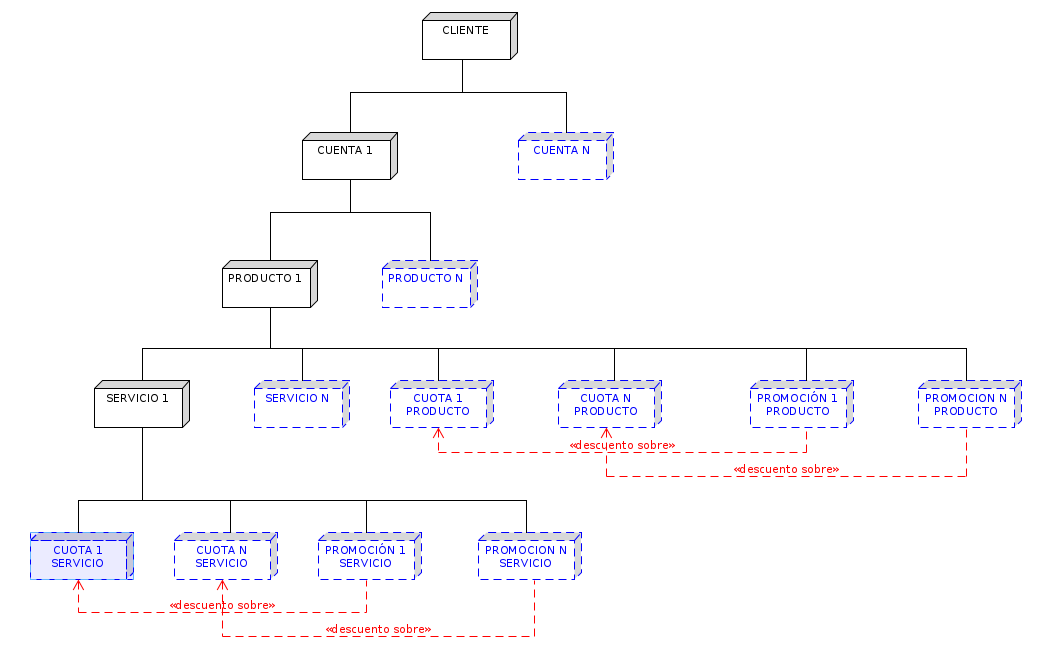
\includegraphics[width=\textwidth]{imaxes/estructura-contratacion.png}
  \caption{Estructura de la contratación}
  \label{fig:estructura-contratacion-chap-teoria}
\end{figure}




\subsubsection{Conceptos relativos al catálogo}
\label{sub:catálogo-conceptos-chap-teoria}


Para llevar a cabo las distintas contrataciones deberemos saber qué características puede tener cada uno de los elementos que intervienen y elegir unas u otras en función de las necesidades que presenta el cliente. Estas características vienen definidas por unas entidades \textit{plantillas} denominadas tipos que se encuentran englobadas dentro de lo que damos en denominar catálogo. 


Un tipo de producto consta de uno o más tipos de servicio con los que puede estar relacionados (relación tipo producto-servicio). 

Sobre ese tipo de producto se define un conjunto de tipos de cuota que pueden aplicar sobre ese tipo de producto (relación tipo producto-cuota).

También sobre ese tipo de producto se define un conjunto de tipos de promoción (relación tipo producto-promoción) que pueden aplicar sobre ese tipo de cuotas asociadas al tipo de producto(relación tipo promoción-cuota).

Por su parte sobre un tipo de servicio se define un conjunto de tipos de cuota que pueden aplicar sobre ese tipo de servicio (relación tipo servicio-cuota).

Y al igual que ocurre con el tipo de producto, sobre ese tipo de servicio se define un conjunto de tipos de promoción (relación tipo servicio-promoción) que pueden aplicar sobre ese tipo de cuotas asociadas al tipo de servicio (relación tipo promoción-cuota) o sobre un tipo de consumos que pueda realizar el servicio (relación tipo promoción-consumo).

A la hora de contratar se selecciona el tipo de producto que se quiera contratar. Las cuotas, servicios y promociones que puedan realizarse en esta contratación vendrán definidos por las relaciones establecidas entre todos esos elementos en el catálogo.


En la \figurename~\ref{fig:estructura-catalogo-chap-teoria} se muestra la estructura que define el catálogo de servicios de la aplicación y como se traslada a una contratación.

\begin{figure}[H]
  \centering
  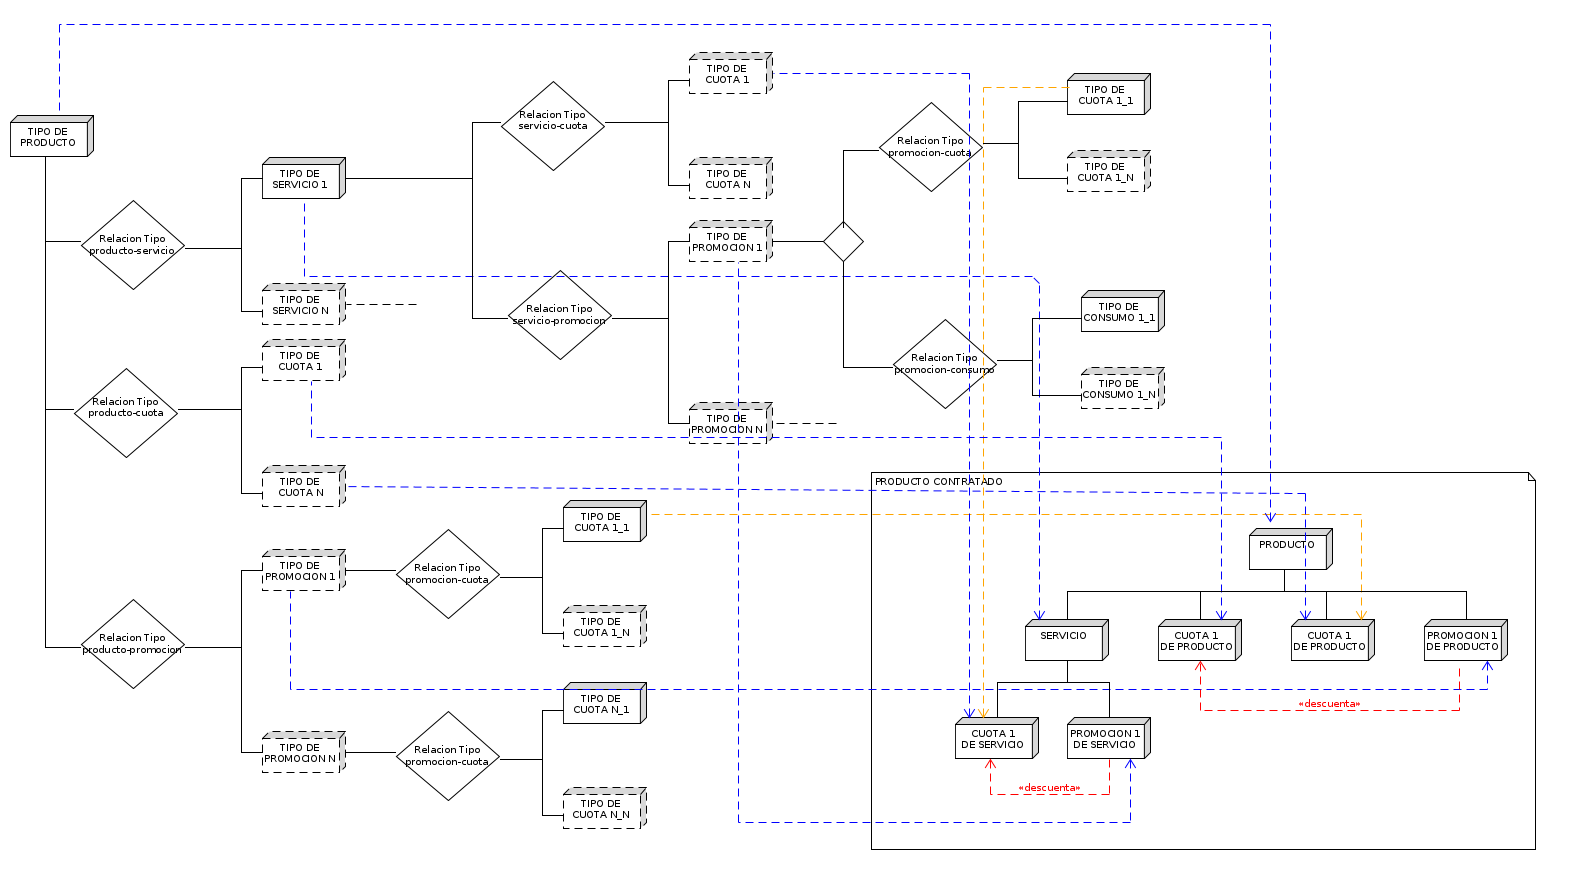
\includegraphics[width=\textwidth]{imaxes/estructura-catalogo.png}
  \caption{Estructura del catálogo de servicios y su implementación en una contratación}
  \label{fig:estructura-catalogo-chap-teoria}
\end{figure}





\subsubsection{Conceptos relativos a los registros de histórico}
\label{sub:histórico-conceptos-chap-teoria}

Puesto que los elementos que conforman las contrataciones son susceptibles de sufrir modificaciones durante su ciclo de vida (nuevas altas de productos, modificación en el precio de las cuotas, expiración de promociones, etc.) todas estas entidades están conformadas por un conjunto de registros históricos que contienen la \textit{foto} de la contratación para el período temporal indicado por las fechas inicio y fin de dicho registro. Lo mismo ocurre con los elementos del catálogo que también pueden sufrir modificaciones en sus condiciones de aplicación, como son las definiciones de cuotas y promociones.

En todos estos casos los registros deben ser consecutivos en el tiempo. Se ha definido los mecanismos necesarios para que la aplicación controle la consecutividad de registros durante las inserciones, modificaciones y borrados pertinentes.